\documentclass{beamer}

\mode<presentation>
{
  \usetheme{Darmstadt}
  \usecolortheme{beaver}
  \usefonttheme{serif}
  \setbeamertemplate{navigation symbols}{}
  \setbeamertemplate{caption}[numbered]
}

\usepackage[english]{babel}
\usepackage[utf8]{inputenc}
\usepackage{booktabs}
\usepackage{amsmath}
\usepackage{graphicx}
\usepackage{animate}
\usepackage{tikz}
\usetikzlibrary{positioning, decorations.pathreplacing, calc}
\graphicspath{{figs/}}

\title[XAI Benchmarking]{Benchmarking Explanation Methods\\on a Multi-Task Vision Transformer}
\author{Nicholas Welsh}
\institute{Florida Institute of Technology\\Department of Computer Science \& Mathematics}
\date{March 2026}

\begin{document}

\begin{frame}
  \titlepage
\end{frame}

\begin{frame}{Outline}
  \tableofcontents
\end{frame}

% ============================================================
\section{Motivation}
% ============================================================

\begin{frame}{Why Explainability?}
\begin{itemize}
  \item Deep networks are powerful but opaque: we cannot easily see \emph{why} a model makes a prediction.
  \item \textbf{Post-hoc explanation methods} produce attribution maps showing which input regions mattered most.
  \item Problem: many methods exist, but how do we know which explanation is ``correct''?
  \item There is no universal ground truth for what a model ``should'' attend to.
\end{itemize}
\vfill
\textbf{Our idea:} Use human gaze data (SALICON) as a quantitative behavioral reference for one dimension of explanation quality.
\end{frame}

\begin{frame}{What Makes This Setup Unique?}
\begin{itemize}
  \item We train a multi-task ViT that \emph{both} classifies images \emph{and} predicts human saliency.
  \item This gives us two kinds of ``where the model looks'':
  \begin{itemize}
    \item The saliency head: what the model \emph{explicitly predicts} humans look at.
    \item XAI methods: what the model \emph{implicitly relies on} for classification.
  \end{itemize}
  \item SALICON fixation maps tell us where humans \emph{actually} look.
  \item We can measure both \textbf{faithfulness} (does masking highlighted regions change the prediction?) and \textbf{human alignment} (do explanations match where people look?).
\end{itemize}
\end{frame}

% ============================================================
\section{Model}
% ============================================================

\begin{frame}{Multi-Task Architecture}
\begin{center}
\resizebox{0.85\linewidth}{!}{%
  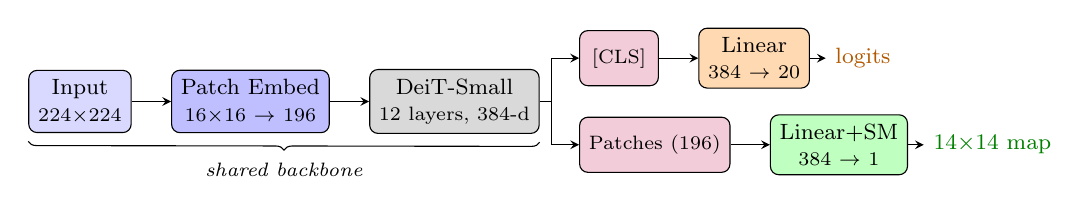
\begin{tikzpicture}[
    node distance=0.5cm,
    box/.style={draw, rounded corners=3pt, minimum height=0.7cm, align=center, font=\footnotesize},
    >=stealth
  ]
    \node[box, fill=blue!15, minimum width=1.3cm] (img)
      {Input\\\scriptsize 224$\times$224};
    \node[box, fill=blue!25, minimum width=1.4cm, right=of img] (patch)
      {Patch Embed\\\scriptsize 16$\times$16 $\to$ 196};
    \node[box, fill=gray!30, minimum width=1.7cm, right=of patch] (backbone)
      {DeiT-Small\\\scriptsize 12 layers, 384-d};
    \node[box, fill=purple!20, minimum width=1.0cm, above right=0.55cm and 0.5cm of backbone.east, anchor=west] (cls)
      {\scriptsize [CLS]};
    \node[box, fill=purple!20, minimum width=1.0cm, below right=0.55cm and 0.5cm of backbone.east, anchor=west] (ptok)
      {\scriptsize Patches (196)};
    \node[box, fill=orange!30, minimum width=1.3cm, right=of cls] (clshead)
      {Linear\\\scriptsize 384 $\to$ 20};
    \node[box, fill=green!25, minimum width=1.3cm, right=of ptok] (salhead)
      {Linear+SM\\\scriptsize 384 $\to$ 1};
    \node[right=0.2cm of clshead, font=\footnotesize, text=orange!70!black] (clsout) {logits};
    \node[right=0.2cm of salhead, font=\footnotesize, text=green!50!black] (salout) {14$\times$14 map};
    \draw[->] (img) -- (patch);
    \draw[->] (patch) -- (backbone);
    \draw[->] (backbone.east) -- ++(0.15,0) |- (cls.west);
    \draw[->] (backbone.east) -- ++(0.15,0) |- (ptok.west);
    \draw[->] (cls) -- (clshead);
    \draw[->] (ptok) -- (salhead);
    \draw[->] (clshead) -- (clsout);
    \draw[->] (salhead) -- (salout);
    \draw[decorate, decoration={brace, amplitude=3pt, mirror}]
      ([yshift=-3pt]img.south west) -- ([yshift=-3pt]backbone.south east)
      node[midway, below=4pt, font=\scriptsize\itshape] {shared backbone};
  \end{tikzpicture}%
}
\end{center}
\begin{itemize}
  \item \textbf{DeiT-Small} (Data-efficient Image Transformer): a ViT trained with an improved recipe on ImageNet-1K without extra data. 12 layers, 384-d, 22M params.
  \item Classification head on CLS token $\rightarrow$ 20 COCO category logits.
  \item Saliency head on patch tokens $\rightarrow$ softmax $\rightarrow$ $14\!\times\!14$ distribution.
  \item Trained with KL divergence for saliency (CC = 0.899, mAP = 0.604).
\end{itemize}
\end{frame}

% ============================================================
\section{Data}
% ============================================================

\begin{frame}{SALICON + COCO}
\begin{itemize}
  \item \textbf{SALICON}: 10,000 train / 5,000 val COCO images with dense fixation maps.
  \item Fixation maps collected via mouse-contingent gaze tracking.
  \item \textbf{COCO 2014}: bounding-box annotations $\rightarrow$ top 20 category labels.
  \item Ground-truth saliency normalized to $14\!\times\!14$ distributions matching the ViT patch grid.
\end{itemize}
\vfill
\small Key advantage: SALICON provides \emph{behavioral} ground truth (thousands of observers), not subjective ratings.
\end{frame}

\begin{frame}{What the Data Looks Like}
\begin{center}
  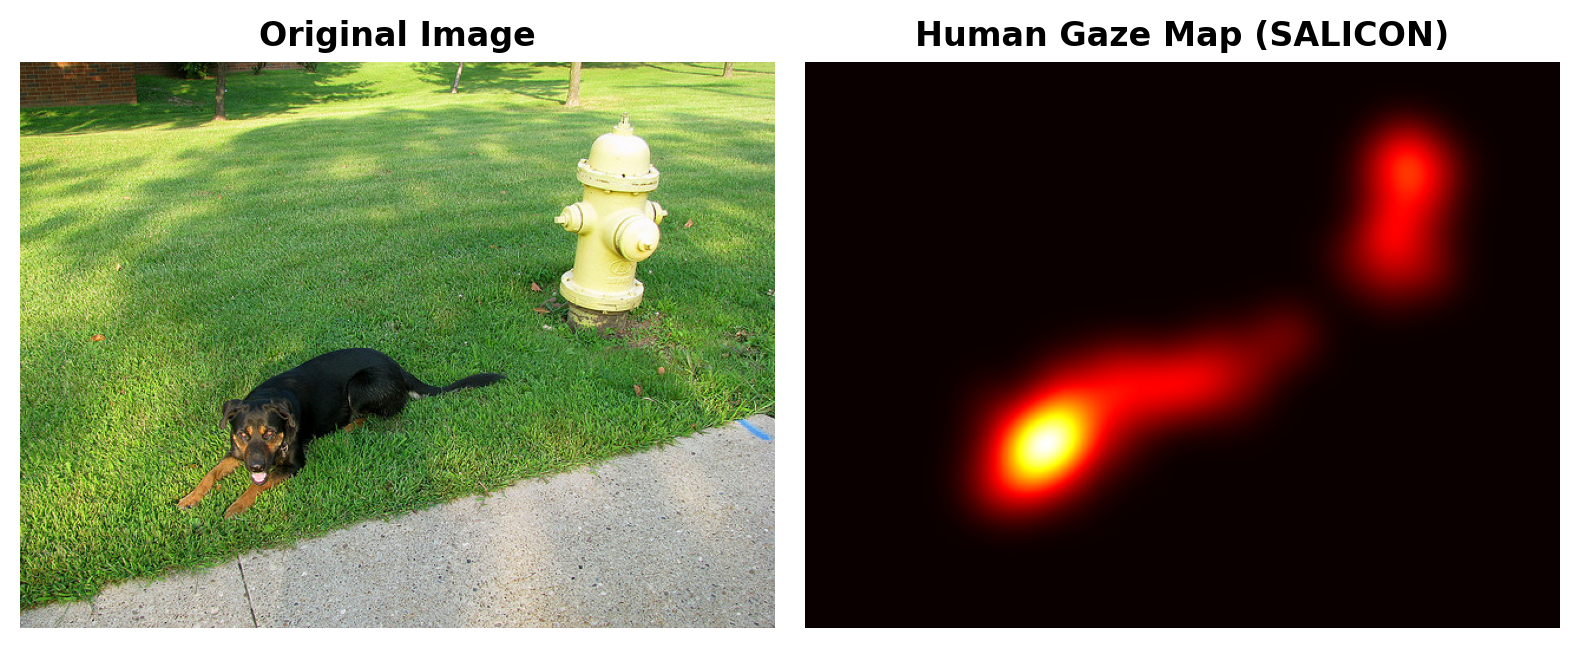
\includegraphics[width=0.95\linewidth]{data_example.png}
\end{center}
\vfill
\small Left: original image. Right: SALICON fixation map showing where thousands of observers looked. This behavioral data serves as our human-alignment reference for evaluating explanations.
\end{frame}

% ============================================================
\section{Explanation Methods}
% ============================================================

\begin{frame}{Gradient-Based Methods}
\small
All explanations computed w.r.t.\ the model's most confident predicted class.
\begin{itemize}
  \item \textbf{Gradient saliency} (Simonyan et al., 2014): $|\partial \ell / \partial x|$, max-pooled across channels. Fast but noisy.
  \item \textbf{Gradient $\times$ input} (Shrikumar et al., 2017): gradient $\odot$ input. Suppresses noise in dark regions.
  \item \textbf{Integrated gradients} (Sundararajan et al., 2017): accumulates gradients from a zero baseline (50 steps). Attributions are guaranteed to sum to the full output difference.
\end{itemize}
\end{frame}

\begin{frame}{Architecture and Perturbation Methods}
\small
\begin{itemize}
  \item \textbf{Attention rollout} (Abnar \& Zuidema, 2020): multiplies attention matrices across 12 layers with residual mixing ($0.5A + 0.5I$). No gradients needed.
  \item \textbf{LIME} (Ribeiro et al., 2016): local linear surrogate on 300 perturbations over a $14\!\times\!14$ patch grid. Model-agnostic.
\end{itemize}
\vfill
\footnotesize Three families: \textbf{gradient} (how sensitive is the output to each pixel?), \textbf{architecture} (where does the model route information?), \textbf{perturbation} (what happens when we hide parts of the input?).
\end{frame}

\begin{frame}{Visual Comparison: Dog + Fire Hydrant}
\begin{center}
  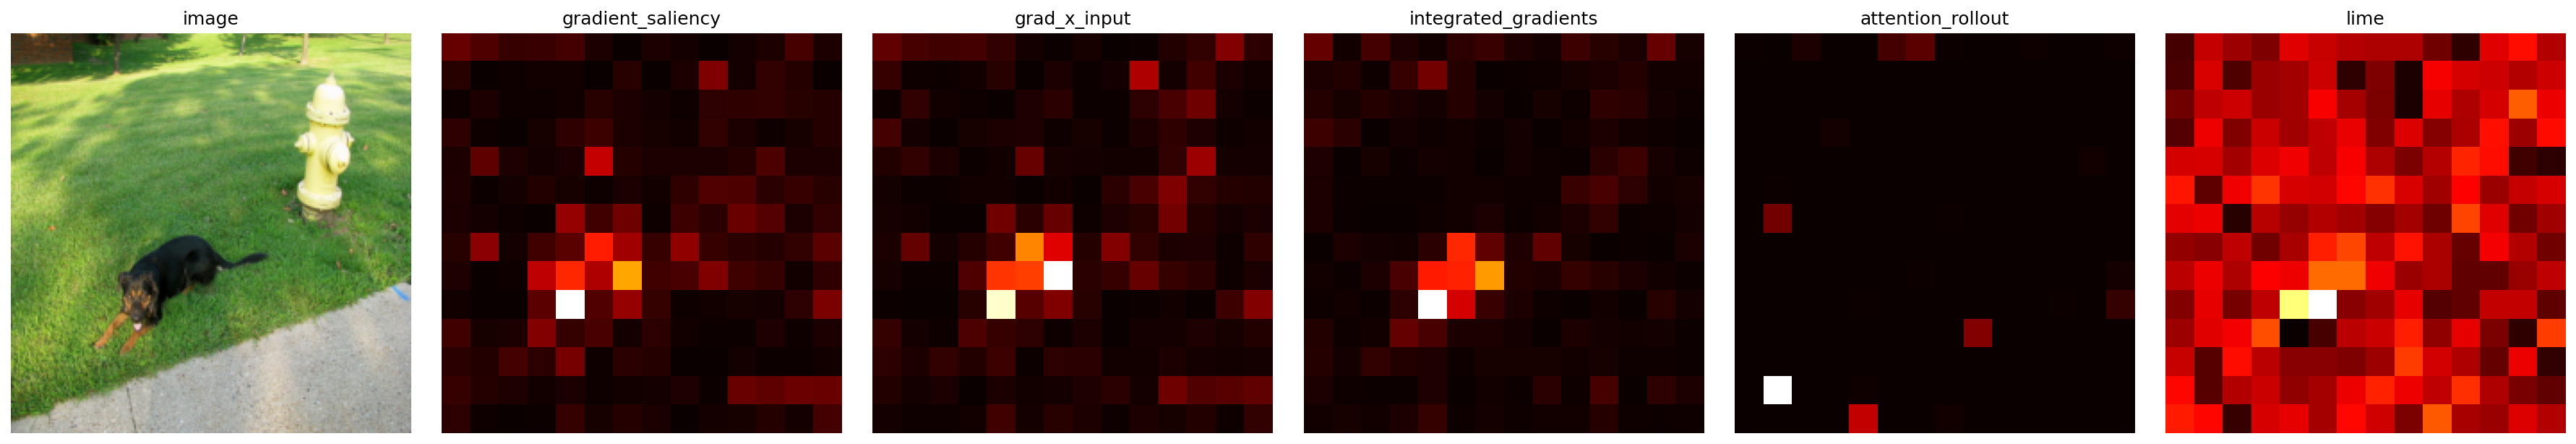
\includegraphics[width=\linewidth]{report_comparison_323.png}
\end{center}
\small Gradient methods highlight the dog. LIME highlights a broader region. Attention rollout collapses to a single bright patch.
\end{frame}

\begin{frame}{Visual Comparison: Tennis Player}
\begin{center}
  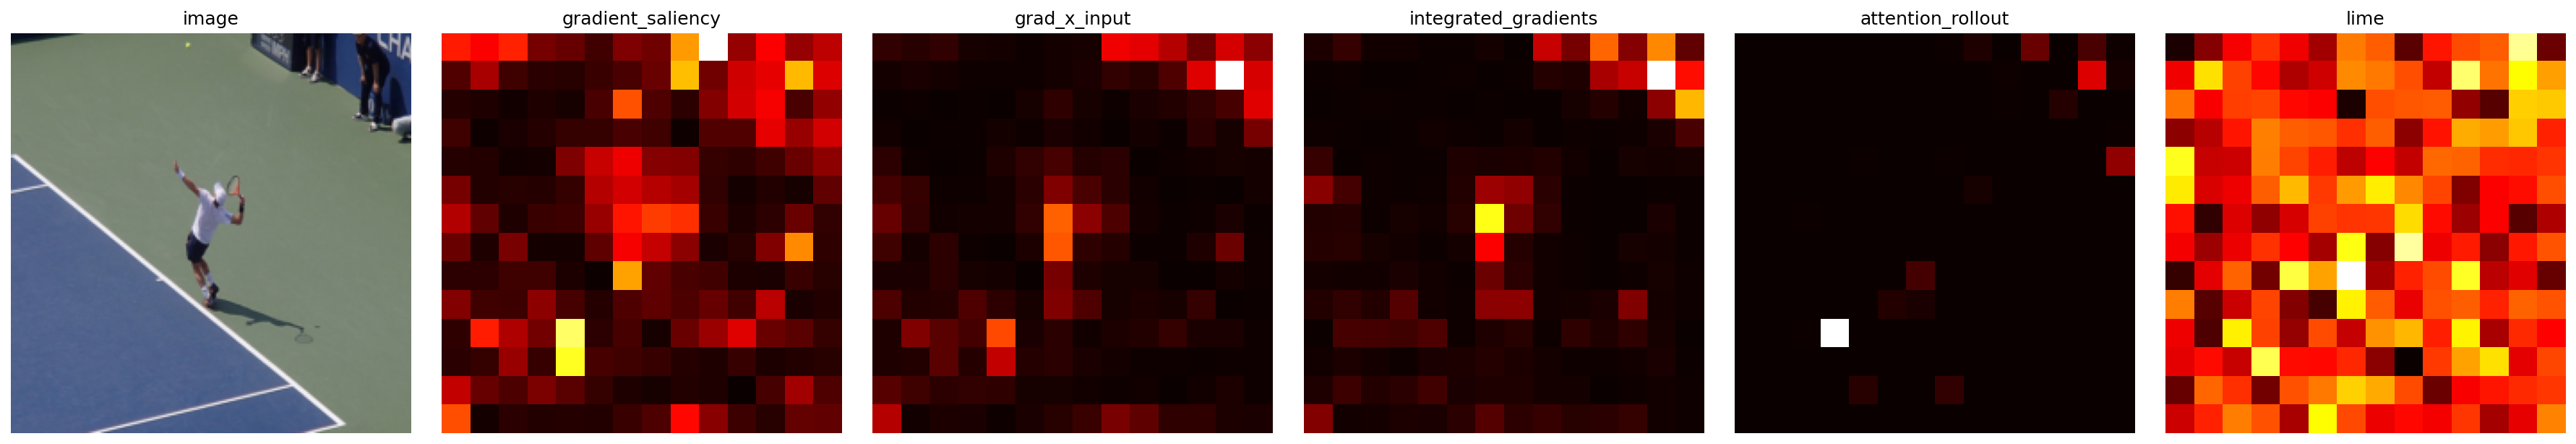
\includegraphics[width=\linewidth]{report_comparison_305.png}
\end{center}
\small Gradient methods agree on the player's location. LIME assigns importance to the court surface, suggesting the model uses background context.
\end{frame}

% ============================================================
\section{Evaluation}
% ============================================================

\begin{frame}{Three Evaluation Axes}
\begin{enumerate}
  \item \textbf{Faithfulness} (does the explanation reflect what the model actually uses?)
  \begin{itemize}
    \item \textbf{Deletion test}: mask patches in importance order, measure confidence drop. Lower AUC = better.
    \item \textbf{Insertion test}: reveal patches in importance order from blank. Higher AUC = better.
  \end{itemize}
  \item \textbf{Stability} (are explanations consistent under small perturbations?)
  \begin{itemize}
    \item Cosine similarity under Gaussian noise, horizontal flip, brightness shift.
  \end{itemize}
  \item \textbf{Human alignment} (does the attribution match where people look?)
  \begin{itemize}
    \item CC and SIM against SALICON fixation maps.
  \end{itemize}
\end{enumerate}
\end{frame}

\begin{frame}{Deletion Test: Live Demo}
\begin{center}
  \animategraphics[autoplay,loop,width=0.9\linewidth]{4}{deletion_frames/frame_}{000}{020}
\end{center}
\vfill
\small Patches are masked in order of attribution importance (Gradient Saliency vs LIME). The confidence curves show how quickly each method identifies decision-critical regions.
\end{frame}

% ============================================================
\section{Results}
% ============================================================

\begin{frame}{Main Results Table}
\begin{center}
\small
\begin{tabular}{lcccc}
\toprule
Method & Del AUC $\downarrow$ & Ins AUC $\uparrow$ & CC $\uparrow$ & SIM $\uparrow$ \\
\midrule
Gradient saliency & 0.468 & 0.766 & 0.161 & 0.410 \\
Grad $\times$ input & 0.521 & 0.768 & 0.171 & 0.405 \\
Integrated gradients & 0.479 & 0.778 & \textbf{0.248} & \textbf{0.434} \\
Attention rollout & 0.544 & 0.745 & $-$0.003 & 0.123 \\
LIME & \textbf{0.409} & \textbf{0.881} & 0.107 & 0.416 \\
\bottomrule
\end{tabular}
\end{center}
\vfill
\begin{itemize}
  \item LIME: best faithfulness, worst human alignment among gradient methods.
  \item Integrated gradients: best human alignment and stability.
  \item Attention rollout: collapses, near-zero alignment.
\end{itemize}
\end{frame}

\begin{frame}{The Central Finding: Faithfulness $\neq$ Human Alignment}
\begin{itemize}
  \item LIME is the most \textbf{faithful} because it directly models the classifier's local decision boundary.
  \item But what the classifier relies on is \emph{not} what humans look at.
  \item The model may use texture, context, or background cues invisible to human inspection.
  \item \textbf{Integrated gradients} strikes the best balance: moderate faithfulness, highest human alignment, highest stability.
\end{itemize}
\vfill
\textbf{Implication:} choosing an XAI method depends on the goal (model debugging vs.\ human communication).
\end{frame}

\begin{frame}{Attention Rollout Collapse}
\begin{itemize}
  \item Attention rollout was designed for shallow transformers.
  \item In DeiT-Small (12 layers), multiplying attention matrices with residual mixing ($0.5A + 0.5I$) causes exponential compounding of CLS-token asymmetry.
  \item Result: rollout concentrates nearly all weight on 1--2 patches regardless of image content.
  \item This is consistent with numerical degeneration in deep attention rollout, not a bug in our code.
  \item CC $\approx -0.003$: no systematic relationship with human gaze.
\end{itemize}
\end{frame}

\begin{frame}{Stability Results}
\begin{center}
\begin{tabular}{lcccc}
\toprule
Method & Noise 0.02 & Noise 0.05 & H-flip & Brightness \\
\midrule
Gradient saliency & 0.963 & 0.918 & 0.768 & 0.988 \\
Integrated gradients & 0.990 & 0.969 & 0.820 & 0.999 \\
\bottomrule
\end{tabular}
\end{center}
\vfill
\begin{itemize}
  \item Integrated gradients is more stable across all perturbation types.
  \item Path integration acts as a smoothing operation, reducing sensitivity to small input changes.
  \item Both methods are highly stable under brightness shifts (DeiT features are intensity-invariant).
\end{itemize}
\end{frame}

% ============================================================
\section{Conclusion}
% ============================================================

\begin{frame}{Key Takeaways}
\begin{enumerate}
  \item \textbf{Faithfulness and human alignment are distinct properties}, even inversely related in some cases.
  \item \textbf{LIME} is the most faithful (best deletion/insertion AUC) but does not match human gaze patterns.
  \item \textbf{Integrated gradients} is the best practical default: moderate faithfulness, best alignment, best stability, axiomatic guarantees.
  \item \textbf{Attention rollout} failed in our DeiT-Small setup, consistent with numerical degeneration of deep matrix products.
  \item \textbf{Method choice depends on use case:} model debugging $\rightarrow$ faithfulness (LIME); human communication $\rightarrow$ alignment (IG).
\end{enumerate}
\end{frame}

\begin{frame}{Limitations and Future Work}
\begin{itemize}
  \item Single model (DeiT-Small) and dataset (SALICON/COCO); results may vary across architectures.
  \item 100-sample evaluation provides stable means but wide per-image variability.
  \item Attribution maps and fixation maps both downsampled to $14\!\times\!14$, which may obscure fine-grained differences.
  \item Future: test on CNNs and larger ViTs, higher-resolution attributions, per-category analysis, additional XAI methods (SmoothGrad, GradCAM).
\end{itemize}
\end{frame}

\begin{frame}
\begin{center}
\Large\textbf{Questions?}

\vfill
\normalsize
Nicholas Welsh \\
\texttt{nwelsh2024@my.fit.edu} \\
\vspace{0.5cm}
\href{https://github.com/nickvpn/vit-ml-xai-project}{github.com/nickvpn/vit-ml-xai-project}
\end{center}
\end{frame}

\end{document}
